% Created 2022-10-31 Mon 15:37
% Intended LaTeX compiler: pdflatex
\documentclass[presentation,aspectratio=1610]{beamer}
\usepackage[utf8]{inputenc}
\usepackage[T1]{fontenc}
\usepackage{graphicx}
\usepackage{grffile}
\usepackage{longtable}
\usepackage{wrapfig}
\usepackage{rotating}
\usepackage[normalem]{ulem}
\usepackage{amsmath}
\usepackage{textcomp}
\usepackage{amssymb}
\usepackage{capt-of}
\usepackage{hyperref}
\usepackage{khpreamble}
\usepackage{pgfplots}
\usepackage{pdfpages}
\usepackage{circuitikz}
\usepgfplotslibrary{groupplots}
\usetikzlibrary{positioning}
\usetikzlibrary{positioning,circuits.plc.ladder}
\renewcommand*{\not}[1]{\ensuremath{\bar{#1}}}
\renewcommand*{\not}[1]{\ensuremath{\overline{#1}}}
\usetheme{default}
\author{Kjartan Halvorsen}
\date{\today}
\title{Programmable Logic Controllers}
\hypersetup{
 pdfauthor={Kjartan Halvorsen},
 pdftitle={Programmable Logic Controllers},
 pdfkeywords={},
 pdfsubject={},
 pdfcreator={Emacs 26.3 (Org mode 9.4.6)}, 
 pdflang={English}}
\begin{document}

\maketitle

\section{Sequential logic}
\label{sec:org7644186}

\begin{frame}[label={sec:orgf264d5f}]{Pressing cheese}
\begin{center}
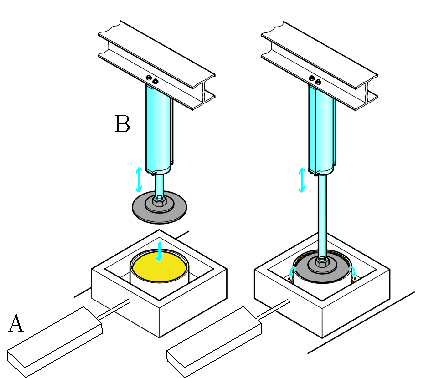
\includegraphics[width=0.5\linewidth]{../../figures/cheese-pressing-two-cylinders}
\end{center}
\end{frame}

\begin{frame}[label={sec:org2329c6a}]{A logic control loop}
\begin{center}
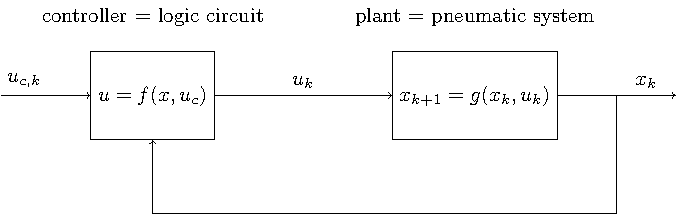
\includegraphics[width=\linewidth]{../../figures/logic-control-loop}
\end{center}
\end{frame}

\begin{frame}[label={sec:org8204abf}]{Pressing cheese}
\begin{columns}
\begin{column}{0.4\columnwidth}
\begin{center}
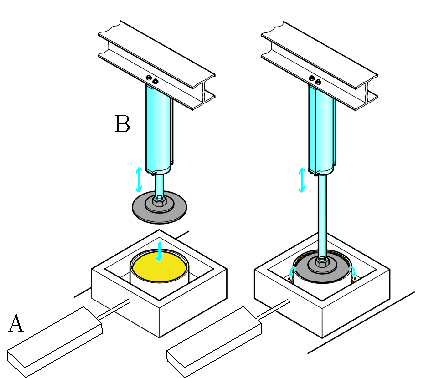
\includegraphics[width=\linewidth]{../../figures/cheese-pressing-two-cylinders}
\end{center}

\pause
\end{column}

\begin{column}{0.6\columnwidth}
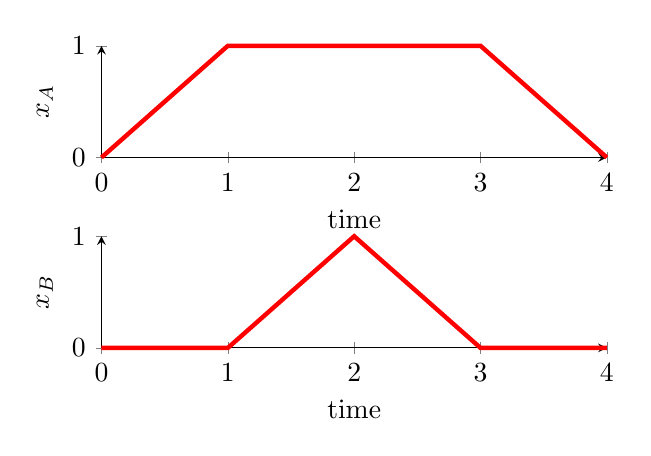
\begin{tikzpicture}
  \begin{groupplot} [
    group style={
      group name=timeplot,
      group size=1 by 3,
      xlabels at=all,
      horizontal sep=1cm,
      vertical sep=1cm,
    }, 
    clip=false,
    height=3cm, width=8cm,
    axis line style={->},
    axis lines=left,
    xlabel={time },
    ylabel={},
    ytick={0,1},
    xtick={0,1,2,3,4},
    % grid=both,
    % xtick=\empty,
    % ytick=\XNOLL,
    % yticklabel=$x_0$,
    ]
    \nextgroupplot [ylabel={$x_A$},]
    \addplot[red, no marks,ultra thick,] coordinates {(0,0) (1,1) (2, 1) (3,1) (4, 0)};
    \nextgroupplot [ylabel={$x_B$},]
    \addplot[red, no marks,ultra thick,] coordinates {(0,0) (1,0) (2, 1) (3,0) (4, 0)};
    %\nextgroupplot [ylabel={$x_P$},]
    %\addplot[red, no marks,ultra thick,] coordinates {(0,0) (1,0) (2, 1) (3,1) (4, 0)};
  \end{groupplot}
\end{tikzpicture}
\end{column}
\end{columns}
\end{frame}


\begin{frame}[label={sec:orgf4930df}]{Pressing cheese}
\begin{columns}
\begin{column}{0.4\columnwidth}
\begin{center}
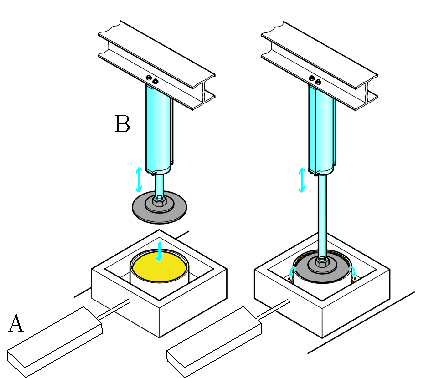
\includegraphics[width=\linewidth]{../../figures/cheese-pressing-two-cylinders}
\end{center}
\end{column}

\begin{column}{0.6\columnwidth}
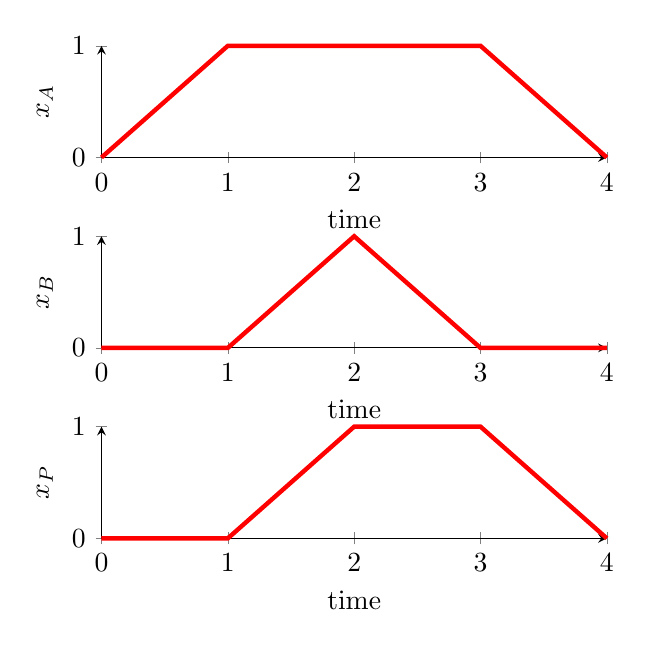
\begin{tikzpicture}
  \begin{groupplot} [
    group style={
      group name=timeplot,
      group size=1 by 3,
      xlabels at=all,
      horizontal sep=1cm,
      vertical sep=1cm,
    }, 
    clip=false,
    height=3cm, width=8cm,
    axis line style={->},
    axis lines=left,
    xlabel={time },
    ylabel={},
    ytick={0,1},
    xtick={0,1,2,3,4},
    % grid=both,
    % xtick=\empty,
    % ytick=\XNOLL,
    % yticklabel=$x_0$,
    ]
    \nextgroupplot [ylabel={$x_A$},]
    \addplot[red, no marks,ultra thick,] coordinates {(0,0) (1,1) (2, 1) (3,1) (4, 0)};
    \nextgroupplot [ylabel={$x_B$},]
    \addplot[red, no marks,ultra thick,] coordinates {(0,0) (1,0) (2, 1) (3,0) (4, 0)};
    \nextgroupplot [ylabel={$x_P$},]
    \addplot[red, no marks,ultra thick,] coordinates {(0,0) (1,0) (2, 1) (3,1) (4, 0)};
  \end{groupplot}
\end{tikzpicture}
\end{column}
\end{columns}
\end{frame}


\section{PLC}
\label{sec:org7396021}
\begin{frame}[label={sec:org840c3d3}]{The Siemens S7 series PLC}
\begin{center}
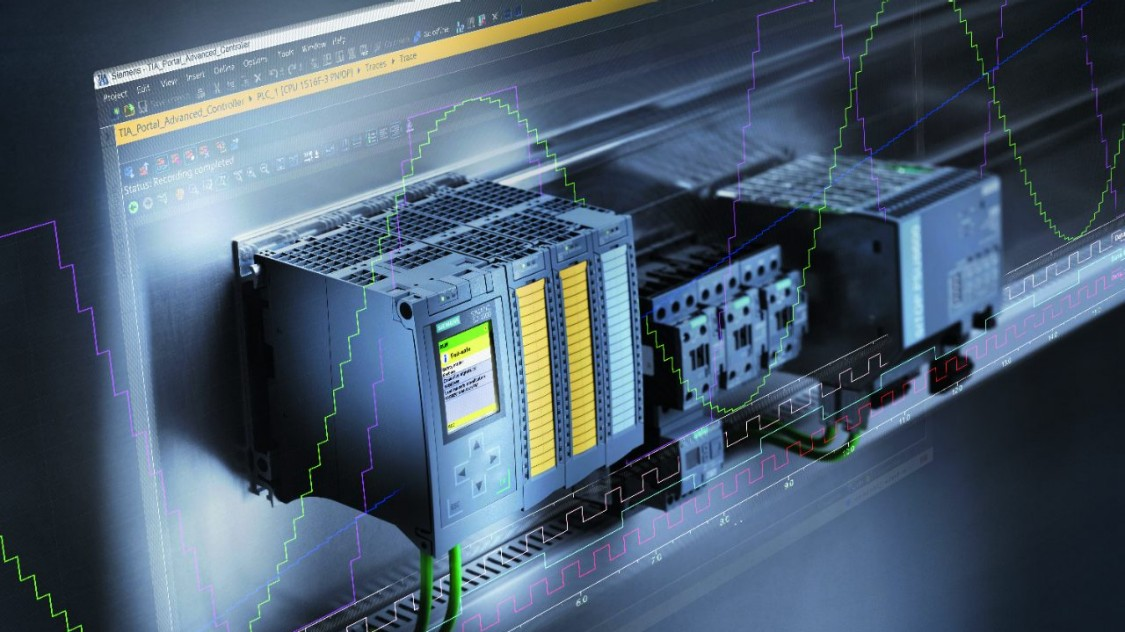
\includegraphics[width=0.8\linewidth]{../../figures/s7-1500.jpeg}
\end{center}

{\footnotesize From Siemens}
\end{frame}


\begin{frame}[label={sec:org367fc65}]{Programming}
Three ways to program the Siemens s7 series
\begin{enumerate}
\item \alert{Ladder diagram (LAD)}
\item Function Block Diagram (FBD)
\item Structured Control Language (SCL)
\end{enumerate}
\end{frame}

\begin{frame}[label={sec:org38445b0}]{Execution}
\begin{center}
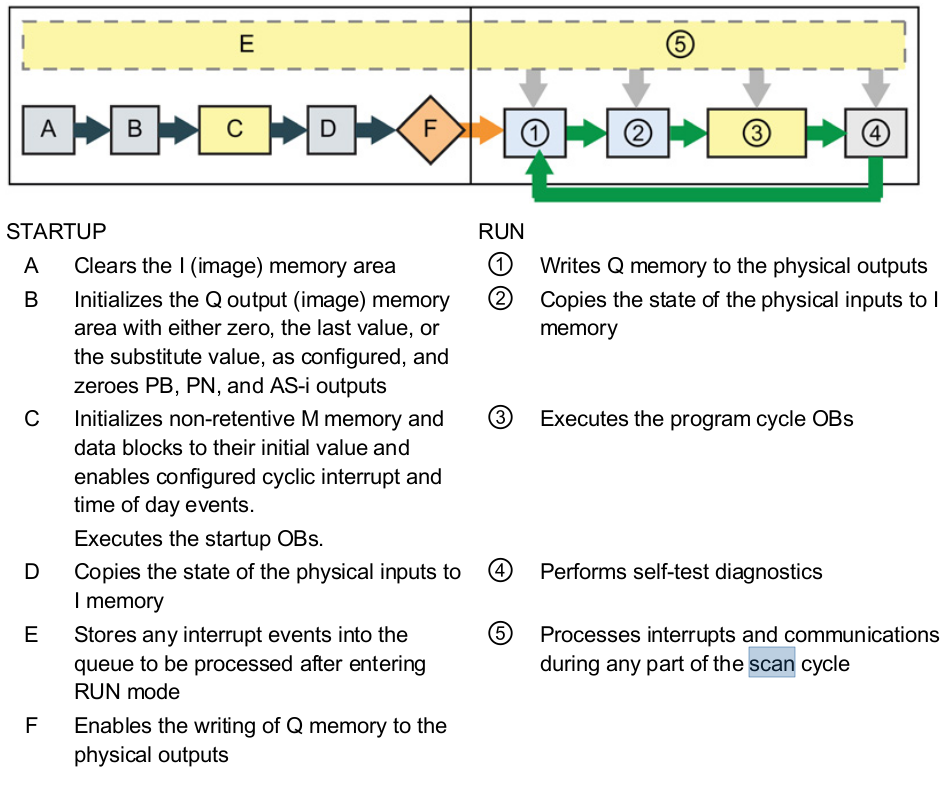
\includegraphics[width=0.7\linewidth]{../../figures/plc-scan.png}
\end{center}
\end{frame}

\section{Ladder diagrams}
\label{sec:org91a243d}
\def\ladderend{12}
\def\rungone{-0.5}
\def\rungtwo{-4.5}
\def\rungthree{-7.5}
\def\relayr{1.5}

\begin{frame}[label={sec:orgabf2d0a}]{PLC Ladder diagrams}
Equivalent to circuit diagram for control logic using relays
\end{frame}

\begin{frame}[label={sec:orgf59c638}]{Basics}
\begin{center}
\begin{tikzpicture}[circuit plc ladder,]
\draw (0,0) to[short, o-]  (0,-2.5);
\draw (\ladderend,0) to[short, o-](\ladderend,-2.5);
\draw (0, \rungone) to[contact NO={info={$X$}},] (2, \rungone) to[ contact NC={info={$Y$}}, ] (4,\rungone) to[short] (6.5, \rungone) to [coil={info={$R$}},] (\ladderend, \rungone) ;
\draw (0, \rungone-\relayr) to[contact NO={info={$R$}},] (2, \rungone-\relayr)  to[short,] (2,\rungone);
\end{tikzpicture}
\end{center}
\end{frame}


\begin{frame}[label={sec:org3db4789}]{A cascade}
\footnotesize
       \begin{center}
       \begin{tikzpicture}[circuit plc ladder, scale=0.8,]
       \draw (0,0) to[short, o-]  (0,-9);
       \draw (\ladderend,0) to[short, o-](\ladderend,-9);
       
       \draw (0, \rungone) to[contact NO={info={$X_1$}},] (2, \rungone) to[contact NO={info={$R_3$}},] (4, \rungone)  to[ contact NC={info={$R_3$}}, ] (6,\rungone)  to [short,] (6.5, \rungone) to [coil={info={$R_1$}},] (\ladderend, \rungone) ;
       \draw (0, \rungone-0.8*\relayr) to[contact NO={info={Start}},] (4, \rungone-0.8*\relayr)  to[short,] (4,\rungone);
       \draw (0, \rungone-1.8*\relayr) to[contact NO={info={$R_1$}},] (4, \rungone-1.8*\relayr)  to[short,] (4,\rungone);

       \draw (0, \rungtwo) to[contact NO={info={$X_2$}},] (2, \rungtwo) to[contact NO={info={$R_1$}},] (4, \rungtwo)  to[ contact NC={info={$R_3$}}, ] (6,\rungtwo)  to [short,] (6.5, \rungtwo) to [coil={info={$R_2$}},] (\ladderend, \rungtwo) ;
       \draw (0, \rungtwo-\relayr) to[contact NO={info={$R_2$}},] (4, \rungtwo-\relayr)  to[short,] (4,\rungtwo);
       
       \draw (0, \rungthree) to[contact NO={info={$X_3$}},] (2, \rungthree) to[contact NO={info={$R_2$}},] (4, \rungthree)  to[ contact NC={info={$R_1$}}, ] (6,\rungthree)  to [short,] (6.5, \rungthree) to [coil={info={$R_3$}},] (\ladderend, \rungthree) ;
       \draw (0, \rungthree-\relayr) to[contact NO={info={$R_3$}},] (4, \rungthree-\relayr)  to[short,] (4,\rungthree);


       \end{tikzpicture}
       \end{center}
\end{frame}
\end{document}